\documentclass[../thesis]{subfiles}

\begin{document}
	\section{Results}
	\label{sec:cuda:results}

	\tdg{intro and method}
	This section presents the efficiency measurements performed for the described \cuda implementation to evaluate how \gpus stand in comparison with the already studied \cpu-only and \intel\xeonphi alternatives. This evaluation follows the methodology described in \cref{sec:case:method}, with a block dimension of 64 (experimentally found to be the best).

	\tdg{HW, SW}
	Results in this section were obtained in \search node 711-1 (already described in \cref{subsec:mic:native:results}), which, in addition to the \intel\xeonphi coprocessor, also contains a \nvidia Tesla K20m board (details in \cref{tab:k20m}). \gcc 4.4.7 and \cuda 5.0 were used to build the test executables.

	\begin{table}
		\centering
		\begin{tabular}{lr}
			\hline
			\gpus & $1\times$ GK110 \\
			Multiprocessors & $13\times$ \smx \\
			\cuda cores & 192 per \smx \\
			Double-precision units & 64 per \smx \\
			\sfus & 32 per \smx \\
			Load/Store units & 32 per \smx \\
			Memory size & 5 GB \\
			\cuda capability & 3.5 \\
			\hline
			Peak DP FLOPS & 1.17 TeraFLOP/s \\
			Peak Memory bandwidth & 208 GB/s \\
			\hline
		\end{tabular}
		\caption{Hardware details for the \nvidia Tesla K20m board in \search node 711-1. Further information available in \cite{NVIDIA:KEPLER,NVIDIA:TeslaKSeriesOverview}.}
		\label{tab:k20m}
	\end{table}

	\tdg{cpu-only is better}
	Although this implementation was able to profit in some measure from the experience gathered in the previous chapters, it was not able to match, much less exceed, the performance obtained in a multicore environment, even before the optimization techniques described in \cref{sec:mic:optims}. \Cref{fig:cuda:results:times} shows the execution times achieved by this (naive) \cuda implementation. The superiority of the multicore implementation is clear, being around 30 times faster for $n=8000$.

	\tdg{reasons for being worse}
	However, there are several reasons for this to happen. First, the multicore implementation has been the target of several optimizations in this document, while this is an initial completely functional \cuda implementation. Given the time already invested in the \intel\xeonphi coprocessor, it is not feasible to perform optimizations targeting the \cuda environment. Next, the absence of optimized \blas and \lapack packages suiting the needs of the implementation. \mkl provides it for both multicore environment and coprocessor, while manual (also naive) implementations had to be devised for \cuda. Lastly, the synchronization requirement between diagonals forces the runtime to return to the \cpu between two consecutive diagonals, creating a bottleneck when the amount of elements/blocks no longer provides enough parallelism to overcome the communication cost.

	\begin{figure}[htp]
		\begin{center}
			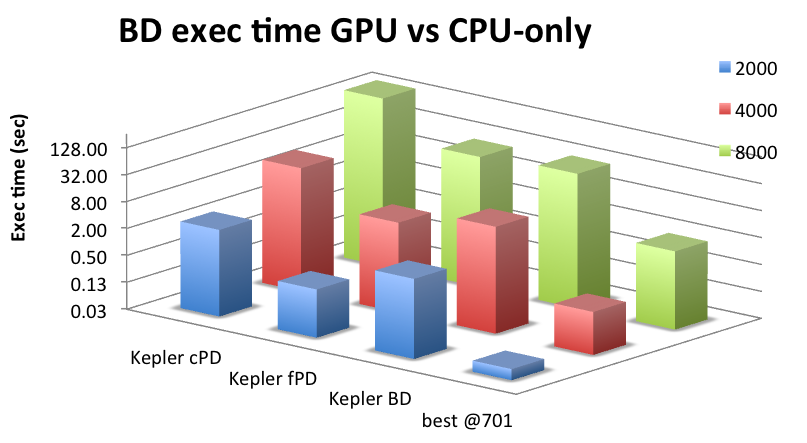
\includegraphics[width=0.9\textwidth]{assets/images/cuda/times.png}
		\end{center}
		\caption{Execution times for the CUDA implementation in a Tesla K20m (Kepler architecture).}
		\label{fig:cuda:results:times}
	\end{figure}
\end{document}

